
\documentclass[11pt, twocolumn]{article}
\usepackage{amsmath}
\usepackage{amsfonts}
\usepackage{mathrsfs}
\usepackage{lscape}
\usepackage{listings}
\usepackage{graphicx} % Allows for importing of figures
\usepackage{color} % Allows for fonts to be colored
\usepackage{comment} % Allows for comments to be made
\usepackage{accents} % Allows for accents to be made above and below text
%\usepackage{undertilde} % Allows for under tildes to take place for vectors and tensors
\usepackage[table]{xcolor}
\usepackage{array,ragged2e}
\usepackage{hyperref}
\usepackage{framed} % Allows boxes to encase equations and such
\usepackage{subcaption} % Allows for figures to be side-by-side
\usepackage{float} % Allows for images to not float in the document
\usepackage{booktabs}
%\usepackage[margin=0.75in]{geometry}
\usepackage[final]{pdfpages}
\usepackage{enumitem}
\usepackage[section]{placeins}
\usepackage{cite}
%%%%%%%%%%%%%%%%%%%%%%%%%  Function used to generate vectors and tensors %%%%%%%%%
\usepackage{stackengine}
\stackMath
\newcommand\tensor[2][1]{%
	\def\useanchorwidth{T}%
	\ifnum#1>1%
	\stackunder[0pt]{\tensor[\numexpr#1-1\relax]{#2}}{\scriptscriptstyle \sim}%
	\else%
	\stackunder[1pt]{#2}{\scriptscriptstyle \sim}%
	\fi%
}
%%%%%%%%%%%%%%%%%%%

\definecolor{mygrey}{rgb}{0.97,0.98,0.99}
\definecolor{codeblue}{rgb}{.2,0,1}
\definecolor{codered}{rgb}{1,0,0}
\definecolor{codegreen}{rgb}{0.3,0.33,0.12}
\definecolor{codegray}{rgb}{0.5,0.5,0.5}
\definecolor{codepurple}{rgb}{0.55,0.0,0.55}
\definecolor{codecyan}{rgb}{0.0,.4,.4}

\lstdefinestyle{mystyle}{
	backgroundcolor=\color{mygrey},   
	commentstyle=\color{codegreen},
	keywordstyle=\color{codeblue},
	stringstyle=\color{codepurple},
	numberstyle=\tiny\color{codegray},
	basicstyle=\footnotesize,
	breakatwhitespace=false,         
	breaklines=true,                 
	captionpos=b,                    
	keepspaces=true, 
	numbers=left,                    
	numbersep=5pt,                  
	showspaces=false,                
	showstringspaces=false,
	showtabs=false,                  
	tabsize=2
}
\lstset{style=mystyle}

\lstset{language=Matlab,backgroundcolor=\color{mygrey}}
\usepackage{lastpage}
\usepackage{fancyhdr}
\pagestyle{fancy}
%%%\lhead{\large{Nik Benko, Peter Creveling}} 
%\chead{\large{\textbf{Automatic Segmentation of Micro CT Images \\  \normalsize{ME EN 6035 Final Project} \\ \small{Nik Benko, Peter Creveling}}}}
%\rhead{\today}
\cfoot{[\thepage\ of \pageref{LastPage}]}
\fancyheadoffset{.5cm}
\setlength{\parindent}{0cm}
\usepackage[left=.5in, right=0.50in, top=1.00in,bottom=1.00in]{geometry}
\usepackage{microtype} 
\usepackage{setspace}
\doublespace
%%%%%%%%%%%%%%%%%%%%%%%%%%%%%%%%%%%%%%%%%%%%%%%%%%%%%%%%%%%%%%%%%%%%%%%%%%
% git testing ii

\begin{document}
\title{ Automatic Segmentation of Micro CT Images  \\ \normalsize{ME EN 6035 Final Project}}
\author{Nik Benko and Peter Creveling}
\maketitle


\begin{abstract} 
In this study, the accuracy of a novel automatic based segmentation pipeline was statistically compared to manual based methods. Segmentation was performed on Fiber-reinforced ceramic matrix composites in order to extract porosity from the surrounding microscturcture. Statistical techniques used to analyze significance included one-way and two-way ANOVA, Tukey's HSD, and 2$\times$2 factorial design. It was found that using a combination of pre-processed filtering, 3D Weka machine learning segmentation, and post-process erosion had the most agreement with manual segmentation.
\end{abstract}

\section{Introduction and Background}

Fiber-reinforced ceramic matrix composites (CMCs) are widely used in the aerospace industry due to their high specific strength and stiffness material properties, and their ability to withstand prolonged exposure to extreme high-temperature and oxidative environments. Despite their increased use, the fundamental physics governing their manufacturing, stochastic microstructure, and long-term structural performance remains largely undiscovered. Understanding the complete life-cycle of CMCs is critical towards improving currently existing and future applications of CMCs. In recent years, the emerging practice of in situ X-ray micro-computed tomography (X-ray $\mu$CT) experiments has proven promising towards providing a holistic understanding into the behavior of CMCs on multiple length scales \cite{Larson,Bale,Bale2,Cox,Haboub,Marshall}.\\
Unique to X-ray $\mu$CT is the ability to image specimens through-thickness in 3-D compared to other surface specific imaging techniques. However, this imaging method comes at a high computational post processing price to analyze terabytes of potential image data. There exist active areas of research in improving best practices for the segmentation of X-ray $\mu$CT reconstructions to extract useful properties. Segmentation is defined as the classification of pixels or groups of pixels into multiple segments. These segments often correspond to a physical representation. There is no one segmentation method that works universally. Segmentation is often tailored towards the users’ needs my means of manual or automatic practices. To date, manual segmentation is heavily used due to the knowledge humans use when classifying individual pixels compared to computer based methods. Once trained, computer based methods significantly out produce humans in computational time, and are therefore more desirable.\\
In this study, a novel segmentation pipeline was developed to accurately segment porosity automatically from the microstructure of CMCs imaged via X-ray $\mu$CT. A statistical validation was performed to compare the differences in segmentation ability of porosity between the novel automatic method and the manual segmentation based method. It was hypothesized that the mean percent error in porosity segmentation for the novel segmentation method was equal to zero under the assumption that the manual based method was considered ground truth. The alternative was the mean percent error in automatic porosity segmentation was greater than zero.


\section{Materials and Methods}

\subsection{Composite CMC and X-ray $\mu$CT}
This study is an extension of current research being performed in the Utah Composites lab where X-ray $\mu$CT is being utilized to image the entire multi-step manufacturing process of CMCs combined with \textit{in situ} testing during extreme environments. The end goal is to fully quantify the changes of the CMC microstructure throughout their entire life-cycle via methods of segmentation. The composite system used consisted of a 8HS satin weave CG Nicalon-fiber fabric infiltrated with SMP-10 resin. Imaging was performed using a Zeiss Versa-520 X-ray CT 3D microscope at the Air Force Research Laboratory (Dayton, OH). In this study, images were analyzed from the pyrolysis step of the manufacturing process after which the resin was cured at 1000$^{\circ}$C.

\subsection{Data}
Image data analyzed was collected after a scan time 37.3 hours from a small region of interest (ROI) from the entire CMC specimen. There were 1980 8-bit images collected with a spatial resolution of 1.21 $\mu$m/voxel. In total, the entire image stack consisted of 22.1GB of information. For this study, a small sub-volume of 500$\times$500$\times$500 pixels analyzed. Within this sub-volume, both manual and automatic segmentation was performed in order to extract porosity (e.g. cracks or voids) from the surrounding microstructure. It is assumed that the manual segmentation based method of porosity is considered ground truth to compare the accuracy of the automatic segmentation.

\subsection{Statistical Analysis} 
Several different statistical techniques were used to evaluate segmentation algorithms. First a one-way ANOVA was conducted on the porosity measurements for each technique to determine whether or not automatic calculations of porosity were significantly different from manual calculations. A multiple comparisons analysis (Tukey's HSD) was then conducted to determine which methods, if any, were significantly different.\\

An additional data set was constructed by calculating the percent error between each of the automatically segmented results and the manually segmented results. This data was no longer dependent on the underlying image and could be treated as a random variable. Normality of data was checked by plotting the histograms for each automatic method. Finally, the four automatic methods segmentations were broken into two categories based on algorithm features with "high" and "low" treatments for each category. A 2 by 2 factorial and 2-way ANOVA were performed to determine which algorithm features (Analysis Dimensions and Edge Erosion), most effected the results. 

\section{Results and Discussion} 
\begin{figure}[H]
	\centering
	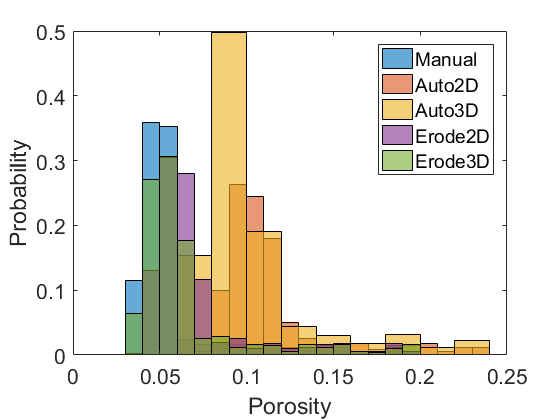
\includegraphics[width=0.5\textwidth]{DataHistograms.png}
	\caption{Histogram of porosity distribution for each segmentation method}
	\label{fig:DataHist}
\end{figure}

\begin{figure}[H]
	\centering
	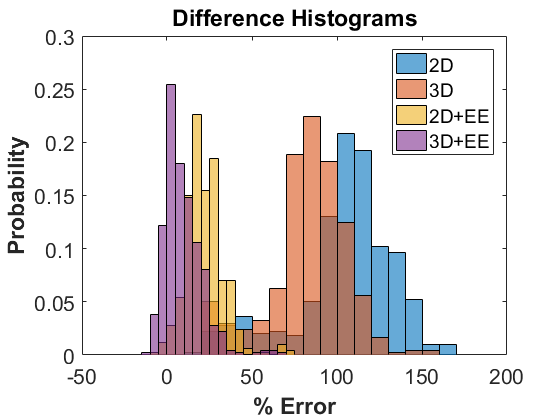
\includegraphics[width=0.5\textwidth]{DifferenceHistograms.png}
	\caption{Histogram of percent error for each of the automatic segmentation methods}
	\label{fig:DiffHist}
\end{figure}

\begin{figure}[H]
	\centering
	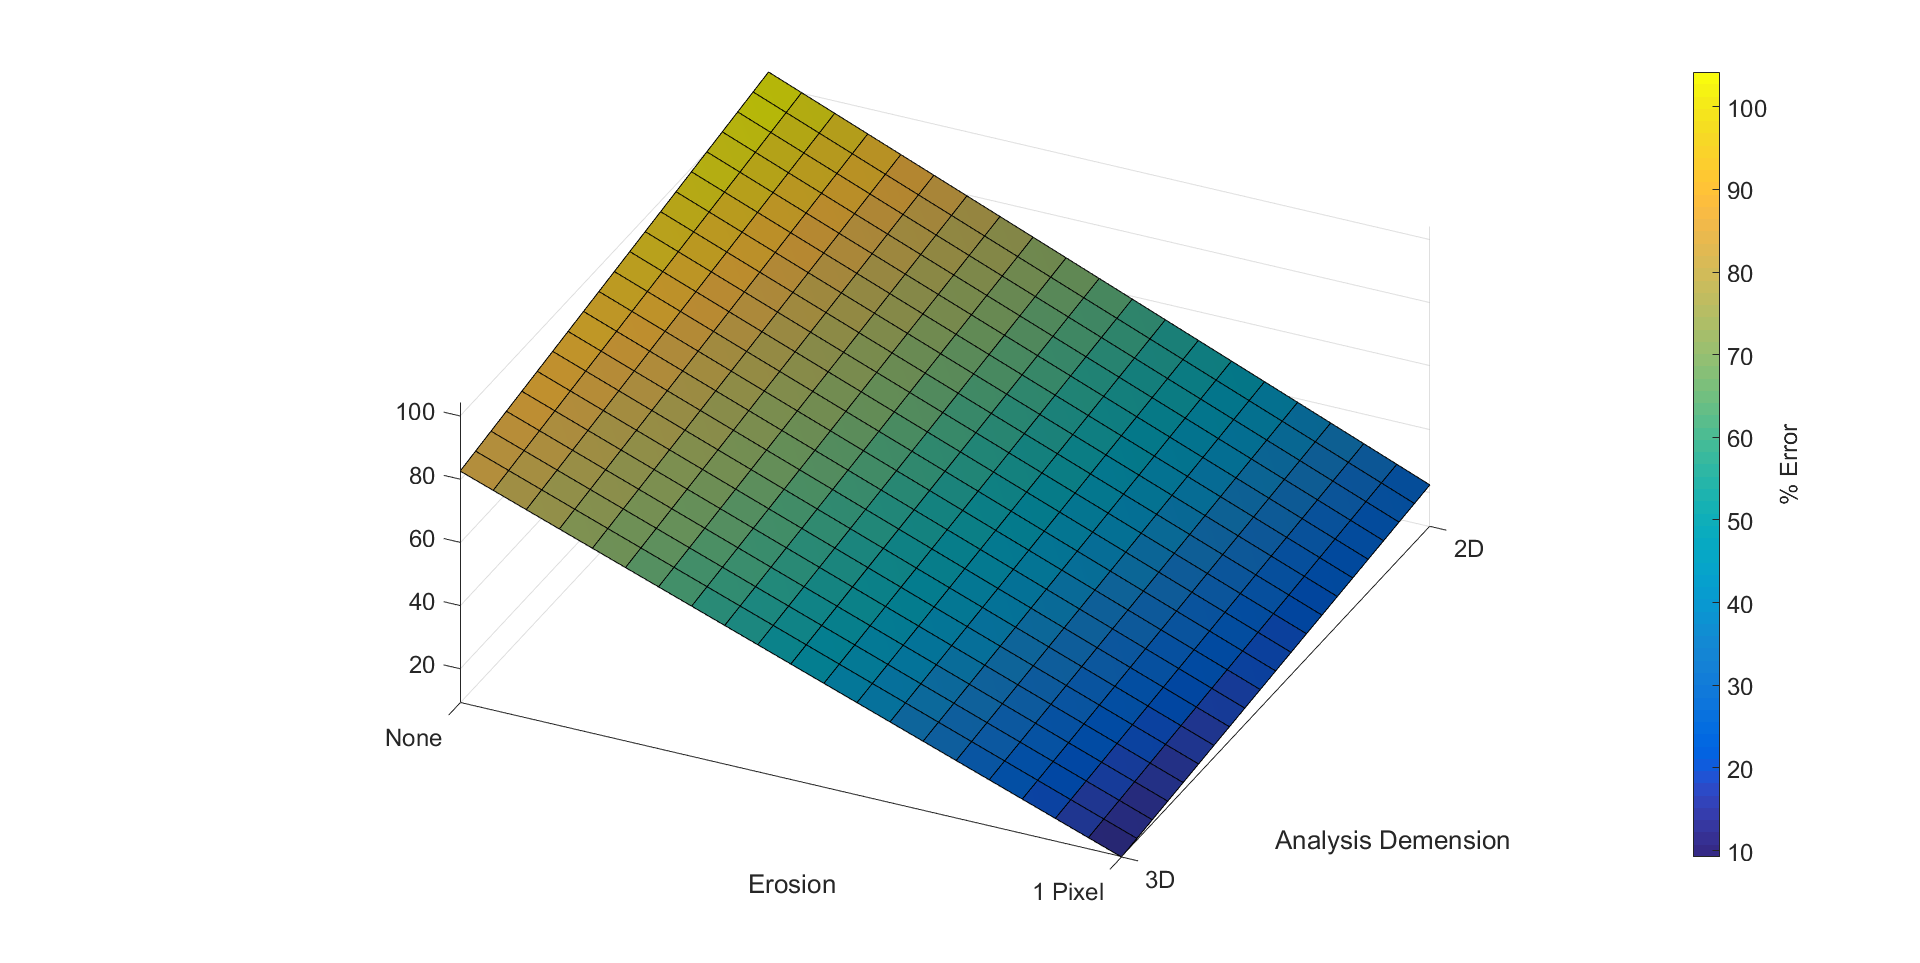
\includegraphics[width=0.5\textwidth]{ResponseSurface.png}
	\caption{Response surface model for two different algorithm features}
	\label{fig:Surf}
\end{figure}
\subsection{Error and Uncertainties} 


\section{Conclusion and Future Directions} 

%\begin{figure}[H]
%	\centering
%	\includegraphics[width=1\textwidth]{TestSetUp.png}
%	\caption{Experimental setup of the Split Hopkinson Pressure Bar}
%	\label{fig:TestSetup}
%\end{figure}


\bibliographystyle{ieeetr}
\bibliography{DoE_References}

\end{document}